% Svolgimento: prova del 01/03/1970, esercizio 1 -- diffrazione di un urto piano attorno a uno spigolo di 105°.
% Numeri e figure: calcoli.py (stessa cartella). Compilare con: latexmk -pdf svolgimento.tex

\documentclass[11pt,a4paper]{article}

\usepackage[T1]{fontenc}
\usepackage[utf8]{inputenc}
\usepackage[italian]{babel}
\usepackage{amsmath,amssymb}
\usepackage[a4paper,margin=2.5cm]{geometry}
\usepackage{array}
\usepackage{siunitx}
\usepackage{booktabs}
\usepackage{graphicx}
\usepackage{float}
\usepackage{caption}
\usepackage{hyperref}

\hypersetup{hidelinks}
\setlength{\parindent}{0pt}
\setlength{\parskip}{4pt}
\allowdisplaybreaks
\graphicspath{{figure/}}
\sisetup{output-decimal-marker={,}, group-separator={\,}, per-mode=symbol,
         exponent-product=\cdot, range-phrase={\text{--}}}

\newcommand{\Cp}{C^{+}}
\newcommand{\Cm}{C^{-}}

\title{Gasdinamica -- Prova del 01/03/1970, esercizio 1\\[2pt]
\large Diffrazione di un urto piano attorno a uno spigolo}
\author{}
\date{}

\begin{document}
\maketitle

\section*{Traccia}
Un urto piano con numero di Mach $M_s=4$ diffrange attorno a uno spigolo vivo C formato da due pareti piane con
angolo di spigolo di $105^\circ$ (schlieren in fig.~\ref{fig:ann}). Davanti all'urto c'è aria in quiete a
$p_1=\SI{1e5}{Pa}$, $T_1=\SI{293}{K}$. Il rapporto fra la posizione della testa A dell'urto diffratto DS (distanza
dall'ascissa di C) e quella del piede B (distanza da C misurata lungo la parete inclinata) vale $2{,}5$. La linea di
separazione SL, che parte da C, ha una prima deviazione $\theta_1=44^\circ$ e una seconda deviazione
$\theta_2=17^\circ$ nel punto F. Si chiede: (a) lo stato dietro l'urto piano prima della diffrazione; (b) la velocità
del piede B; (c) l'intensità del ventaglio di Prandtl--Meyer centrato in C, perché c'è e perché il suo fronte di testa
termina in D; (d) l'intensità del ventaglio centrato in F; (e) l'intensità dell'urto di ricompressione RC, perché c'è
e la sua geometria; (f) perché c'è la discontinuità di contatto CD e perché va dal punto E, che si muove lungo la
parete inclinata come il piede dell'urto, fino a D; (g) le linee di corrente in tutto il campo; (h) la deviazione
della linea di separazione in C nel campo asintotico.

%==============================================================================
\section{Lettura del testo e dell'immagine}
La schlieren rende visibili i gradienti di densità: gli urti sono linee chiare, nette e sottili; i ventagli di
espansione sono zone a luminosità graduata; il contatto è una linea più debole e sfumata. L'immagine è un'istantanea
di un fenomeno \textbf{instazionario}: l'urto piano, partito da sinistra, ha superato lo spigolo C (la linea verticale
sottile per C ne segna la posizione all'istante del passaggio, $t=0$) e si sta propagando verso destra in aria in
quiete. Dietro l'urto il gas si muove verso destra (frecce ``streamlines''). La parete superiore del condotto è il
bordo nero in alto; il blocco nero in basso a sinistra è il corpo, con la faccia orizzontale a monte di C e la faccia
inclinata che scende da C verso B, ruotata di $105^\circ$ rispetto alla corrente.

Non c'è una scala delle lunghezze, ma non serve: la traccia dà un rapporto fra distanze e, come mostro al
§\ref{sec:scorciatoie}, nel campo le distanze da C sono proporzionali alle velocità. Il gas è aria, gas ideale con
$\gamma=1{,}4$ e $R=\SI{287}{J/(kg.K)}$. La traccia è identica a quella del 13/02/2023 (B70-E01 del catalogo).

\begin{figure}[H]
  \centering
  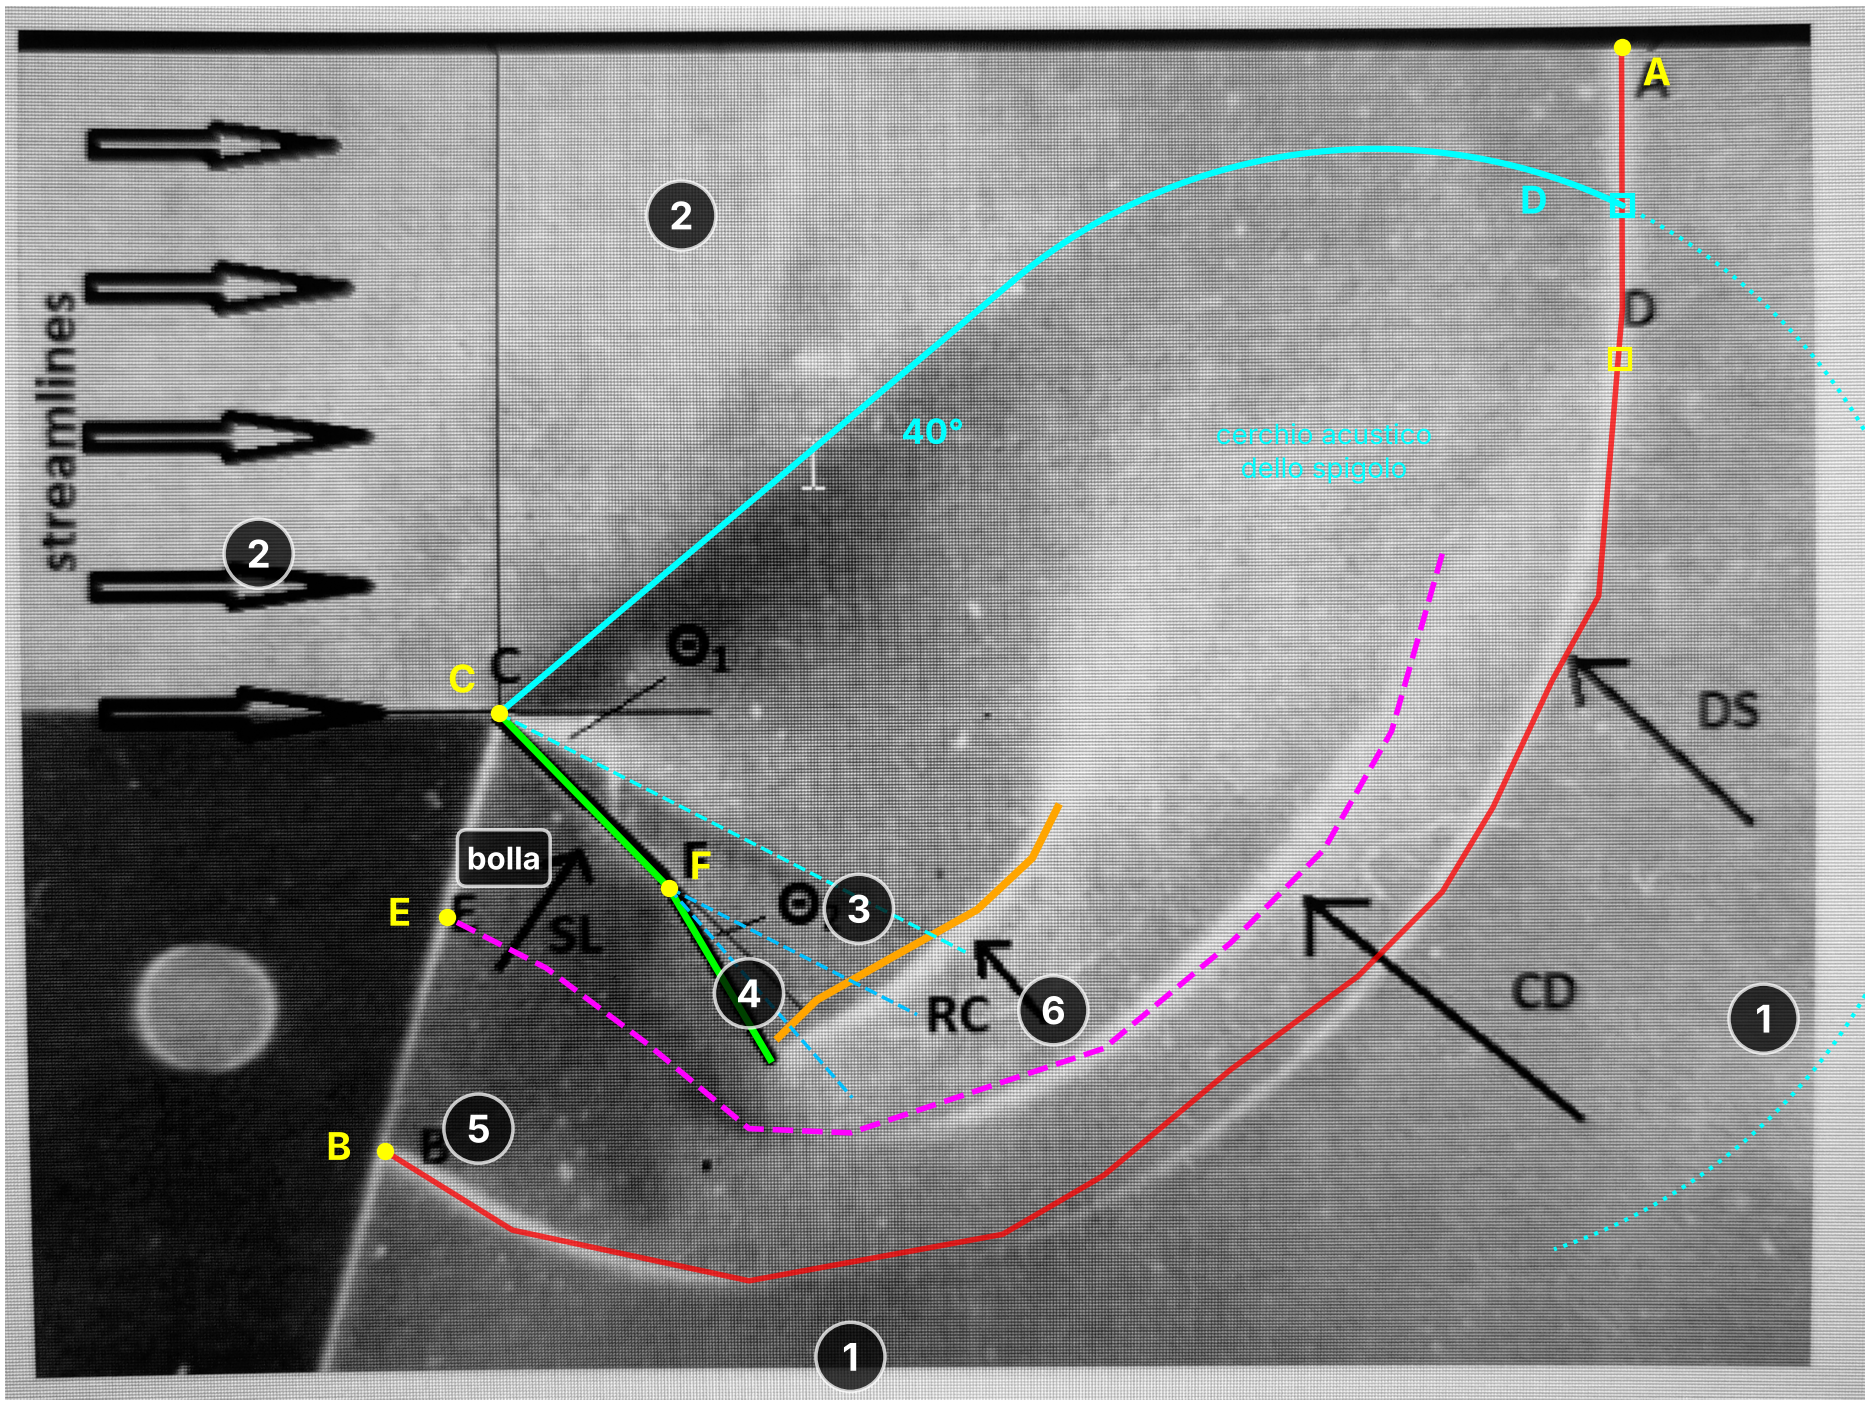
\includegraphics[width=0.92\textwidth]{annotata.png}
  \caption{Schlieren con le strutture identificate. Rosso: urto diffratto DS (da A a B); ciano: fronte di testa del
  ventaglio centrato in C (tratto rettilineo inclinato di $\mu_2$ fino alla tangenza con il cerchio acustico dello
  spigolo, poi l'arco di cerchio fino a D sull'urto piano; il quadratino ciano è il punto D calcolato, quello giallo
  il punto da cui la curvatura di DS diventa visibile); tratteggio ciano: code dei ventagli in C e in F; verde: linea
  di separazione SL con lo spigolo F; arancio: urto di ricompressione RC; magenta: discontinuità di contatto CD, da D
  fino a E sulla parete inclinata. I numeri indicano gli stati.}
  \label{fig:ann}
\end{figure}

%==============================================================================
\section{Identificazione delle strutture}
\begin{itemize}
  \item \textbf{DS, urto diffratto} (linea chiara esterna, da A a B). Fra A e D è ancora l'urto piano, perpendicolare
  alla parete superiore; sotto D si incurva e si indebolisce scendendo verso la parete inclinata, che raggiunge
  perpendicolarmente nel piede B. Resta sottile in ogni suo punto perché è un'onda di compressione: le
  caratteristiche vi convergono e la mantengono discontinua.
  \item \textbf{Ventaglio di Prandtl--Meyer centrato in C} (zona scura che parte da C verso l'alto a destra). Il suo
  bordo superiore è rettilineo e passa per C: è la testa del ventaglio, una linea di Mach della corrente 2. La
  luminosità varia gradualmente, come in un'espansione isentropica.
  \item \textbf{SL, linea di separazione} (tratto nero spezzato C--F--fine). La corrente non segue la parete
  inclinata: si stacca nello spigolo vivo C e lo strato di scorrimento delimita una \textbf{bolla} di gas lento fra SL
  e la parete. In F la linea devia ancora e termina in un vortice (macchia scura sotto la fine di SL).
  \item \textbf{Ventaglio centrato in F}: è l'espansione legata alla seconda deviazione di SL; non si distingue da
  quella in C, perché i due ventagli sono contigui.
  \item \textbf{RC, urto di ricompressione} (bordo netto fra la zona scura e quella chiara, dalla fine di SL verso
  l'alto a destra). È netto in basso e sfuma salendo, dentro il ventaglio di C.
  \item \textbf{CD, discontinuità di contatto} (seconda linea chiara, fra RC e DS, più debole di DS). È più marcata in
  basso e sfuma salendo verso D; in basso si chiude verso il vortice e la parete inclinata, nel punto E.
  \item Il disco chiaro nel blocco nero e le frecce sono elementi della stampa, non del campo.
\end{itemize}

%==============================================================================
\section{Ipotesi e modello}
\begin{itemize}
  \item \textbf{Eulero 2D piano, instazionario}, gas ideale con $\gamma$ costante; fuori dallo strato di scorrimento SL
  e dal vortice trascuro la viscosità. Le strutture nette dell'immagine (urti, ventagli) sono quelle di un campo non
  viscoso; SL e la bolla invece sono effetti viscosi, e la loro geometria la prendo dai dati (deviazioni $\theta_1$,
  $\theta_2$).
  \item \textbf{Campo autosimile} (pseudo-stazionario): spigolo vivo, pareti piane e stati iniziali uniformi non
  danno alcuna lunghezza di riferimento, quindi la soluzione dipende solo da $x/t$, $y/t$. L'immagine a un istante
  successivo sarebbe la stessa, ingrandita in proporzione al tempo trascorso dal passaggio dell'urto in C.
  \item \textbf{Vicino allo spigolo la corrente è stazionaria}: in un campo autosimile un punto a distanza fissa da C
  ha $r/t\to0$, cioè assume lo stato del centro della similitudine; la corrente 2 che arriva su C è uniforme e, come
  verificherò, supersonica. Quindi in C nasce un \textbf{ventaglio di Prandtl--Meyer stazionario}, e lo stesso in F.
  \item \textbf{Linea di separazione come contorno a pressione assegnata}: attraverso SL la pressione è continua, e su
  ogni tratto rettilineo la corrente esterna è uniforme; le deviazioni $\theta_1$ e $\theta_2$ sono quindi le
  deviazioni dei due ventagli.
  \item \textbf{Piede dell'urto perpendicolare alla parete} (lo si vede in B): il gas davanti è in quiete e dietro un
  urto la velocità indotta è normale all'urto; perché sia tangente alla parete, l'urto deve essere normale alla
  parete. In B il piede è quindi un urto normale piano che corre lungo la parete nel gas 1.
\end{itemize}

%==============================================================================
\section{Misure sull'immagine}
Misuro con righello e goniometro, prendendo C come origine.
\begin{itemize}
  \item Distanza di A dall'ascissa di C e distanza CB lungo la parete inclinata: rapporto $\approx 2{,}5$, come dice il
  testo; la parete inclinata forma $\approx 105^\circ$ con la direzione della corrente.
  \item Inclinazione del bordo della zona scura che parte da C (testa del ventaglio): $\approx 40^\circ$ sopra
  l'orizzontale.
  \item SL: primo tratto a $\approx 46^\circ$, secondo a $\approx 59^\circ$ sotto l'orizzontale; entro la precisione
  della lettura concordano con $\theta_1=44^\circ$ e $\theta_1+\theta_2=61^\circ$, e nel calcolo uso i dati del testo.
  \item Punto E: $\mathrm{CE}/\mathrm{CB}\approx 0{,}47$.
  \item RC: distanza di C dalla tangente a RC nel suo tratto basso, $h_{RC}\approx 0{,}37\,x_A$; lì RC è quasi
  perpendicolare alla corrente che lo attraversa.
  \item Punto in cui la curvatura di DS diventa visibile: altezza $\approx 0{,}32\,x_A$ sopra C.
\end{itemize}

%==============================================================================
\section{Analisi qualitativa e topologia del campo}
\textbf{Prima dello spigolo.} L'urto piano mette in moto verso destra il gas in quiete. Dietro un urto in gas in
quiete la corrente è supersonica quando $M_s\gtrsim 2{,}07$: con $M_s=4$ la corrente 2 è supersonica rispetto alla
parete, e questo decide tutta la struttura vicino a C.

\textbf{Allo spigolo.} La corrente 2 arriva su uno spigolo convesso: si espande in un ventaglio di Prandtl--Meyer
centrato in C (onde $\Cp$, perché la parete è sotto la corrente: i fronti salgono e la corrente ruota in senso orario).
Non può seguire una rotazione di $105^\circ$: si separa e la bolla fissa la deviazione ($\theta_1$, poi $\theta_2$
in F). Le perturbazioni partite da C raggiungono l'urto piano, perché questo è subsonico rispetto al gas che ha dietro
($|M_r|<1$): l'urto si incurva sotto D e si indebolisce scendendo (DS), fino al piede B, che corre lungo la parete
inclinata nel gas in quiete con un'intensità molto minore di quella dell'urto piano.

\textbf{Più a valle.} La corrente espansa (stati 3 e 4) ha pressione molto minore di quella del gas messo in moto da
DS; deve ricomprimersi e, essendo supersonica rispetto alle strutture, lo fa con un urto, RC. Il gas passato
dall'urto piano e quello passato soltanto per DS, più debole, hanno entropie diverse: li separa il contatto CD.

\textbf{Stati} (fig.~\ref{fig:ann}):
\begin{itemize}
  \item 1: gas in quiete davanti a DS;
  \item 2: dietro l'urto piano, uniforme; sopra la testa del ventaglio di C e fuori dal cerchio acustico dello
  spigolo;
  \item 3: dopo il ventaglio di C, lungo il primo tratto di SL ($\theta=-44^\circ$); è una striscia fra la coda del
  ventaglio di C e la testa di quello di F, che sono parallele;
  \item 4: dopo il ventaglio di F, lungo il secondo tratto di SL ($\theta=-61^\circ$);
  \item 5: dietro il piede B, fra DS e CD vicino alla parete inclinata;
  \item 6: dietro RC; non uniforme, perché RC è attraversato da stati diversi;
  \item bolla: gas lento fra SL e la parete inclinata, con il vortice alla fine di SL.
\end{itemize}
Le zone fra RC, CD e DS non sono uniformi (DS è curvo): basta descriverle, senza risolverle.

%==============================================================================
\section{Scorciatoie fisiche}\label{sec:scorciatoie}
\textbf{Autosimilarità.} Ogni struttura parte da C all'istante $t=0$ e il campo dipende solo da $x/t$, $y/t$: ogni
punto riconoscibile si muove a velocità costante, proporzionale alla sua distanza da C. Quindi il rapporto fra due
distanze misurate è il rapporto fra le velocità, con la scala data dalla testa A, che è l'urto piano e corre a $W$:
\[
  \frac{W_B}{W} = \frac{\mathrm{CB}}{x_A}.
\]
Per un'onda curva conta la velocità normale: il punto di un'onda autosimile in cui la normale è $\mathbf n$ si sposta,
lungo $\mathbf n$, di $h=\mathbf r\cdot\mathbf n$ in un tempo $t$, dove $h$ è la distanza di C dalla tangente
all'onda; quindi $W_n=h/t=W\,h/x_A$.

\textbf{Stazionarietà vicino a C.} Per lo stesso motivo il campo vicino allo spigolo è stazionario: lì valgono le
relazioni di Prandtl--Meyer e, per $t\to\infty$, è quello il \textbf{campo asintotico} chiesto in (h).

%==============================================================================
\section{Calcolo}

\subsection*{a) Stato 2, dietro l'urto piano}
\[
  a_1=\sqrt{\gamma R T_1}=\SI{343}{m/s},\qquad W = M_s a_1 = \SI{1373}{m/s}.
\]
Nel riferimento dell'urto il gas 1 entra con Mach $M_s$: valgono le relazioni dell'urto normale con $M_1=M_s$;
tornando al laboratorio, $u_2 = W - v_2 = W(1-\rho_1/\rho_2)$:
\[
  \frac{p_2}{p_1}=1+\frac{2\gamma}{\gamma+1}\,(M_s^2-1)=18{,}5,\qquad
  \frac{\rho_2}{\rho_1}=\frac{(\gamma+1)M_s^2}{(\gamma-1)M_s^2+2}=4{,}57,\qquad
  u_2=\frac{2a_1}{\gamma+1}\Big(M_s-\frac{1}{M_s}\Big).
\]
\begin{gather*}
  p_2=\SI{18.5e5}{Pa},\qquad T_2=T_1\,\frac{p_2}{p_1}\frac{\rho_1}{\rho_2}=\SI{1186}{K},\\
  u_2=\SI{1072}{m/s},\qquad a_2=\SI{690}{m/s},\qquad M_2=\frac{u_2}{a_2}=1{,}55.
\end{gather*}
Grandezze totali della corrente 2 (servono per i ventagli): $p_{02}=p_2\,(1+\delta M_2^2)^{\gamma/(\gamma-1)}=
\SI{73.4e5}{Pa}$, $T_{02}=\SI{1758}{K}$, con $\delta=(\gamma-1)/2$.

\subsection*{b) Velocità del piede B e stato 5}
Dall'autosimilarità, con il rapporto dato:
\[
  W_B=\frac{W}{2{,}5}=\SI{549}{m/s},\qquad M_B=\frac{W_B}{a_1}=1{,}60 .
\]
Il piede è un urto normale che corre lungo la parete nel gas in quiete (stesse relazioni del punto a):
\begin{gather*}
  \frac{p_5}{p_1}=2{,}82,\qquad \frac{\rho_5}{\rho_1}=2{,}03,\qquad T_5=\SI{407}{K},\\
  u_5=\frac{2a_1}{\gamma+1}\Big(M_B-\frac{1}{M_B}\Big)=\SI{279}{m/s},\qquad a_5=\SI{404}{m/s},\qquad M_5=0{,}69 .
\end{gather*}
Il gas 5 si muove lungo la parete inclinata, verso B, ed è subsonico.

\subsection*{c) Ventaglio centrato in C: stato 3}
\textbf{Perché c'è.} La corrente 2 è supersonica ($M_2=1{,}55$) e vicino a C stazionaria; lo spigolo convesso la
costringe a ruotare in senso orario, e la rotazione di una corrente supersonica attorno a uno spigolo convesso, senza
una lunghezza di riferimento, è un ventaglio centrato di onde $\Cp$.

Attraverso le onde $\Cp$ si conserva $\theta+\nu$; la corrente ruota di $\theta_1$, quindi
\[
  \nu(M_3)=\nu(M_2)+\theta_1,\qquad \nu(M_2)=\SI{13.5}{\degree}\ \Rightarrow\ \nu(M_3)=\SI{57.5}{\degree},\ M_3=3{,}44 .
\]
L'espansione è isentropica ($p_0$ costante):
\[
  p_3=p_2\,\frac{(1+\delta M_2^2)^{\gamma/(\gamma-1)}}{(1+\delta M_3^2)^{\gamma/(\gamma-1)}}=\SI{1.06e5}{Pa},
  \qquad \frac{p_3}{p_2}=0{,}057 ,
\]
\[
  T_3=\SI{523}{K},\quad a_3=\SI{459}{m/s},\quad V_3=M_3a_3=\SI{1575}{m/s},\quad \theta_3=-44^\circ .
\]
L'intensità del ventaglio è quindi una deviazione di $44^\circ$ con un rapporto di pressione $p_3/p_2=0{,}057$. Fronte
di testa: linea di Mach della corrente 2, inclinata di $\mu_2=\arcsin(1/M_2)=\SI{40.1}{\degree}$ sopra l'orizzontale;
coda: $\theta_3+\mu_3=\SI{-27.1}{\degree}$.

\textbf{Perché la testa termina in D.} La prima perturbazione partita da C (all'istante $t=0$) si propaga con il
suono nel gas 2 che la trasporta: al tempo $t$ è un cerchio di centro $u_2t$ (sull'orizzontale di C) e raggio $a_2t$,
e le perturbazioni successive stanno dentro l'inviluppo formato dalla linea di Mach per C tangente al cerchio e dal
cerchio stesso. La testa del ventaglio è quindi rettilinea solo fino alla tangenza, a distanza
$\sqrt{u_2^2-a_2^2}\,t=821\,t$ da C, e poi prosegue lungo il cerchio. Il cerchio raggiunge l'urto piano perché
$u_2+a_2>W$ (l'urto è subsonico rispetto al gas 2: $|M_r|=(W-u_2)/a_2=0{,}43$). Il punto d'incontro è D:
\[
  (W-u_2)^2+y_D^2=a_2^2 \ \Rightarrow\ \frac{y_D}{x_A}=\frac{\sqrt{a_2^2-(W-u_2)^2}}{W}=0{,}45 .
\]
Sopra D l'urto non ha ancora ricevuto alcuna informazione dello spigolo e resta piano, con lo stato 2 dietro; sotto D
diffrange. Il fronte di testa del ventaglio, cioè il confine della zona perturbata dallo spigolo, termina quindi
sull'urto in D.

\subsection*{d) Ventaglio centrato in F: stato 4}
In F la linea di separazione devia ancora di $\theta_2$: la pressione nella bolla vicino al vortice è più bassa che
vicino a C, e la corrente vi si adatta con una seconda espansione centrata, di onde $\Cp$:
\[
  \nu(M_4)=\nu(M_3)+\theta_2=\SI{74.5}{\degree}\ \Rightarrow\ M_4=4{,}75,\qquad
  p_4=\SI{0.187e5}{Pa},\quad \frac{p_4}{p_3}=0{,}177,\quad \frac{p_4}{p_2}=0{,}010,
\]
\[
  T_4=\SI{319}{K},\quad a_4=\SI{358}{m/s},\quad V_4=\SI{1700}{m/s},\quad \theta_4=-61^\circ .
\]
Testa a $\theta_3+\mu_3=\SI{-27.1}{\degree}$, parallela alla coda del ventaglio di C, coda a
$\theta_4+\mu_4=\SI{-48.9}{\degree}$.

\subsection*{e) Urto di ricompressione RC: stato 6}
\textbf{Perché c'è.} Dopo le due espansioni la corrente è a $p_4\approx\SI{0.19e5}{Pa}$ (e $p_3\approx\SI{1.1e5}{Pa}$
più in alto), mentre il gas messo in moto da DS è a pressioni fra $p_5=\SI{2.8e5}{Pa}$ (al piede) e
$p_2=\SI{18.5e5}{Pa}$ (vicino a D). Attraverso CD la pressione è continua: la corrente espansa deve ricomprimersi.
Rispetto alle strutture, che si spostano molto più lentamente di essa, è supersonica e non può ricevere l'informazione
da valle in modo graduale: si ricomprime con un urto.

\textbf{Geometria.} I ventagli sono centrati in C e in F, quindi la corrente espansa esce quasi radialmente dallo
spigolo; l'urto che la ricomprime le è quasi perpendicolare ed è un arco concavo verso C. Parte dalla fine di SL,
dove la corrente è nello stato 4 e la differenza di pressione è massima, quindi lì è più intenso; salendo entra nel
ventaglio di C, dove la corrente è sempre meno espansa ($M\to M_2$, $p\to p_2$), si indebolisce e svanisce come onda
di Mach: è ciò che si vede nella schlieren, dove RC è netto in basso e sfuma in alto. Per l'autosimilarità RC si
allontana da C con velocità normale
\[
  W_{RC}=W\,\frac{h_{RC}}{x_A}\approx\SI{510}{m/s}\approx W_B ,
\]
poiché RC dista da C circa quanto B. Prendo quindi $W_{RC}\approx W_B$ e RC normale alla corrente a monte: nel
riferimento di RC la corrente arriva con Mach relativo
\[
  M_{r}=\frac{V-W_{RC}}{a}:\qquad
  M_{r4}=\frac{V_4-W_B}{a_4}=3{,}22,\qquad M_{r3}=\frac{V_3-W_B}{a_3}=2{,}24 ,
\]
e le relazioni dell'urto normale danno l'intensità
\[
  \frac{p_6}{p_4}=1+\frac{2\gamma}{\gamma+1}(M_{r4}^2-1)=11{,}9\ \Rightarrow\ p_6\approx\SI{2.2e5}{Pa}\ \text{(tratto basso)},
\]
\[
  \frac{p_6}{p_3}=1+\frac{2\gamma}{\gamma+1}(M_{r3}^2-1)=5{,}7\ \Rightarrow\ p_6\approx\SI{6.0e5}{Pa}\ \text{(tratto centrale)},
\]
e $p_6/p\to1$ all'estremo superiore, dove RC svanisce. Con il valore misurato di $W_{RC}$ invece di $W_B$, $p_6$
cambia di meno del 10\%: la stima è robusta. Dietro RC la corrente è subsonica rispetto all'urto (Mach relativo
$\approx0{,}46$ e $0{,}55$).

\subsection*{f) Contatto CD e punto E}
Il gas fra CD e DS è stato messo in moto da DS dopo il passaggio in C; quello all'interno di CD è il gas che era già
stato attraversato dall'urto piano ($M_s=4$) prima della diffrazione e che poi ha girato lo spigolo (ventagli, RC,
bolla). Attraverso CD pressione e velocità normale sono continue, ma l'entropia no: l'urto piano ha prodotto
$\Delta s/R=1{,}98$, mentre DS, che si indebolisce da $M\approx4$ in D a $M_B=1{,}6$ in B, produce un salto di entropia
che va da quello dell'urto piano fino a $\Delta s/R=0{,}11$ al piede. Il salto di entropia attraverso CD, e quindi di
densità e di temperatura, è nullo in D, dove l'urto è ancora quello piano: per questo CD si ferma in D e sfuma salendo
verso D. È massimo in basso, dove CD tocca la parete in E.

E è un punto di un contatto, cioè materiale: sta sulla parete e si muove con il gas a parete, cioè con la velocità $u_5$
del gas dietro il piede. Anche E, come B, corre lungo la parete a velocità costante (campo autosimile), e il rapporto
delle distanze da C deve essere quello delle velocità:
\[
  \frac{\mathrm{CE}}{\mathrm{CB}}=\frac{u_5}{W_B}=0{,}51\quad\text{(misurato: }\approx0{,}47).
\]

\subsection*{g) Linee di corrente}
Le linee di corrente istantanee (fig.~\ref{fig:lc}) si ricavano dalla direzione della velocità in ogni zona:
\begin{itemize}
  \item nella zona 2, fuori dalla zona perturbata dallo spigolo, sono orizzontali e arrivano così fino al tratto piano
  A--D di DS, dove terminano: davanti a DS il gas è fermo;
  \item quelle che entrano nel ventaglio di C si incurvano verso il basso; in un ventaglio centrato la portata fra due
  raggi si conserva, $\rho a\,r=\text{cost}$, quindi la distanza da C cresce molto e la rotazione avviene in un tratto
  lungo: solo le linee vicine a SL completano la rotazione di $44^\circ$ (stato 3) e poi quella di $17^\circ$ in F
  (stato 4);
  \item attraversano RC senza cambiare direzione (RC è quasi normale alla corrente) e rallentano; attraversano CD e
  arrivano a DS perpendicolarmente, perché dietro un urto che entra nel gas in quiete la velocità è normale all'urto;
  \item la linea di parete si separa in C lungo SL, devia in F e si avvolge nel vortice; nella bolla il gas ricircola
  (scende lungo SL trascinato dallo strato di scorrimento e risale lungo la parete verso C);
  \item da E verso B il gas scorre lungo la parete inclinata con velocità $u_5$, fino al piede, dove la velocità è
  parallela alla parete e normale all'urto; vicino a DS le linee arrivano normali all'urto.
\end{itemize}

\begin{figure}[H]
  \centering
  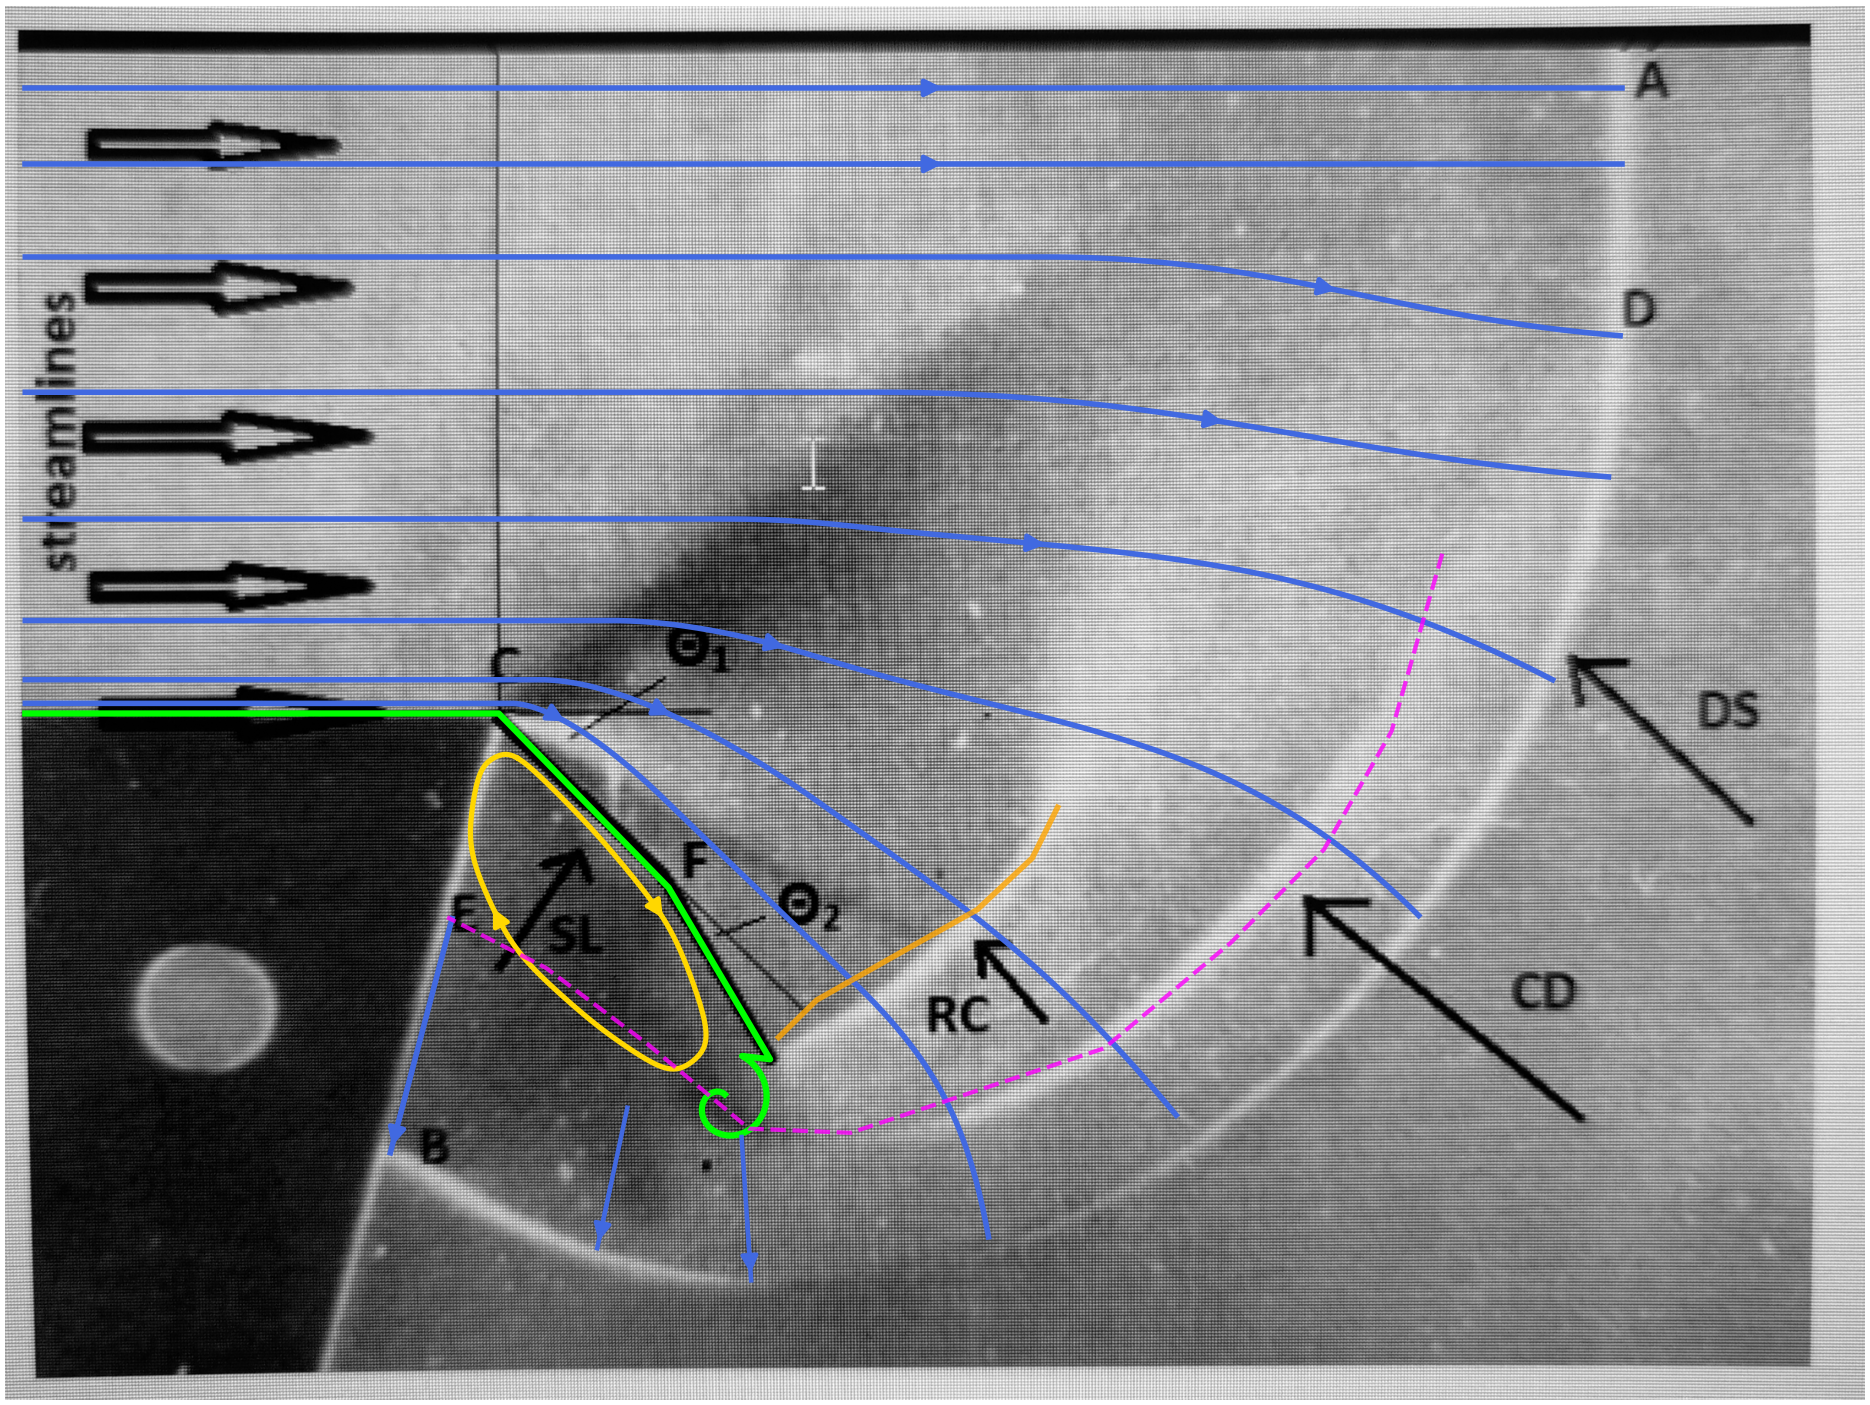
\includegraphics[width=0.86\textwidth]{linee_corrente.png}
  \caption{Linee di corrente istantanee (blu) nel riferimento del laboratorio; verde: linea di separazione e vortice;
  giallo: ricircolo nella bolla; arancio: RC; magenta: CD. Le linee che arrivano su DS vi terminano perpendicolarmente
  (gas fermo davanti all'urto).}
  \label{fig:lc}
\end{figure}

\subsection*{h) Campo asintotico: deviazione della linea di separazione in C}
Per $t\to\infty$ l'urto si allontana e allo spigolo resta la corrente stazionaria che esce dal condotto (stato 2) e si
espande nell'ambiente a $p_1$: la bolla, a contatto con l'ambiente, ne assume la pressione, e la linea di separazione,
contorno a pressione assegnata, devia di quanto serve a portare la corrente 2 a $p_1$ con un'espansione isentropica:
\begin{gather*}
  \frac{p_{02}}{p_1}=(1+\delta M_\infty^2)^{\gamma/(\gamma-1)}=73{,}4\ \Rightarrow\ M_\infty=3{,}47,\\
  \nu(M_\infty)=\SI{58.1}{\degree},\qquad \theta_\infty=\nu(M_\infty)-\nu(M_2)=\SI{44.6}{\degree}.
\end{gather*}
È la prima deviazione misurata, $\theta_1=44^\circ$: infatti $p_3\approx\SI{1.06e5}{Pa}\approx p_1$. Non è un caso:
il campo vicino a C è già quello asintotico (§\ref{sec:scorciatoie}), e la bolla vicino allo spigolo è già alla
pressione dell'ambiente.

%==============================================================================
\section{Verifiche}
\begin{itemize}
  \item Corrente 2 supersonica: $M_2=1{,}55>1$ (serve $M_s>2{,}07$), quindi il ventaglio stazionario in C è
  ammissibile. Verificata.
  \item Urto piano subsonico rispetto al gas dietro: $|M_r|=0{,}43<1$, quindi le perturbazioni di C raggiungono l'urto e
  D esiste. Verificata.
  \item Piede: $M_B=1{,}60>1$ e $\Delta s>0$; è più debole dell'urto piano ($p_5<p_2$), come deve essere per un urto che
  si indebolisce diffrangendo. Verificata.
  \item Testa del ventaglio: misurata $\approx40^\circ$, calcolata $\mu_2=40{,}1^\circ$. Verificata.
  \item Geometria: rapporto A/B misurato $\approx2{,}5$, parete a $\approx105^\circ$, come nel testo. Verificata.
  \item Ventagli: $\nu(M_4)=74{,}5^\circ<\nu_{max}=130{,}5^\circ$ e $p_0$ costante; deviazione totale di SL
  $61^\circ<105^\circ$, quindi SL non tocca la parete e la bolla esiste. Verificata.
  \item RC: $M_{r}>1$ in entrambi i tratti, quindi è un urto di compressione con $\Delta s>0$; le pressioni dietro RC
  ($\approx2{,}2$--$\SI{6.0e5}{Pa}$) stanno fra quelle del gas dietro DS nelle zone corrispondenti
  ($p/p_1\approx2{,}8$--$8$, vedi la discussione), coerente con la continuità di pressione attraverso CD.
  Verificata in ordine di grandezza.
  \item E: $\mathrm{CE}/\mathrm{CB}\approx0{,}47$ misurato contro $u_5/W_B=0{,}51$. Verificata.
  \item Campo asintotico: $\theta_\infty=44{,}6^\circ\approx\theta_1$ e $p_3\approx p_1$. Verificata.
  \item D: calcolato a $y_D\approx0{,}45\,x_A$; la curvatura di DS si vede solo da $\approx0{,}32\,x_A$. È coerente: in
  D arriva una perturbazione infinitesima (acustica), quindi l'urto inizia a curvarsi con pendenza continua e la
  curvatura diventa visibile solo più in basso.
\end{itemize}

%==============================================================================
\section{Risultati}
\begin{table}[H]
  \centering
  \small
  \begin{tabular}{lll}
    \toprule
    Grandezza & Valore & \\
    \midrule
    Stato 2 & $p_2=\SI{18.5e5}{Pa}$, $T_2=\SI{1186}{K}$, $u_2=\SI{1072}{m/s}$, $M_2=1{,}55$ & esatto \\
    Piede B & $W_B=\SI{549}{m/s}$, $M_B=1{,}60$, $p_5=\SI{2.82e5}{Pa}$, $u_5=\SI{279}{m/s}$ & esatto (dati) \\
    Ventaglio in C & $\Delta\theta=44^\circ$, $M_3=3{,}44$, $p_3/p_2=0{,}057$, $p_3=\SI{1.06e5}{Pa}$ & esatto (dati) \\
    Ventaglio in F & $\Delta\theta=17^\circ$, $M_4=4{,}75$, $p_4/p_3=0{,}177$, $p_4=\SI{0.19e5}{Pa}$ & esatto (dati) \\
    RC & $p_6/p_4\approx12$ ($p_6\approx\SI{2.2e5}{Pa}$), $p_6/p_3\approx5{,}7$ ($p_6\approx\SI{6.0e5}{Pa}$) & stima \\
    D & $y_D/x_A=0{,}45$ & esatto \\
    Campo asintotico & $\theta_\infty=44{,}6^\circ\approx\theta_1$ & esatto \\
    \bottomrule
  \end{tabular}
  \caption{Risultati richiesti. ``Esatto (dati)'': esatto nel modello, a partire dai valori misurati dati nel testo.}
\end{table}

%==============================================================================
\section{Rappresentazioni}
Le deviazioni della corrente lungo SL e le pressioni si leggono nel piano $p$--$\theta$ (fig.~\ref{fig:pt}): la curva
è l'espansione $\Cp$ isentropica dallo stato 2 ($p_0=p_{02}$), su cui stanno 3 ($\theta=-44^\circ$), 4
($\theta=-61^\circ$) e il punto asintotico $\infty$, dove la curva taglia $p=p_1$, quasi coincidente con 3. RC è
normale alla corrente: non cambia la direzione, quindi è un salto verticale da 4 e da 3 ai due valori di $p_6$. Lo
stato 5 sta alla direzione della parete inclinata ($\theta=-105^\circ$). Le pressioni vanno da quasi
$\SI{2e6}{Pa}$ a $\SI{2e4}{Pa}$, due ordini di grandezza: la scala logaritmica mostra tutti gli stati e la curva
che, per deviazioni oltre $80^\circ$, scende verso il vuoto; quella lineare mostra quanto la pressione crolli già nei
primi $40^\circ$ di rotazione, e che dopo RC il gas torna a pressioni dell'ordine di $p_5$, molto sotto $p_2$.

\begin{figure}[H]
  \centering
  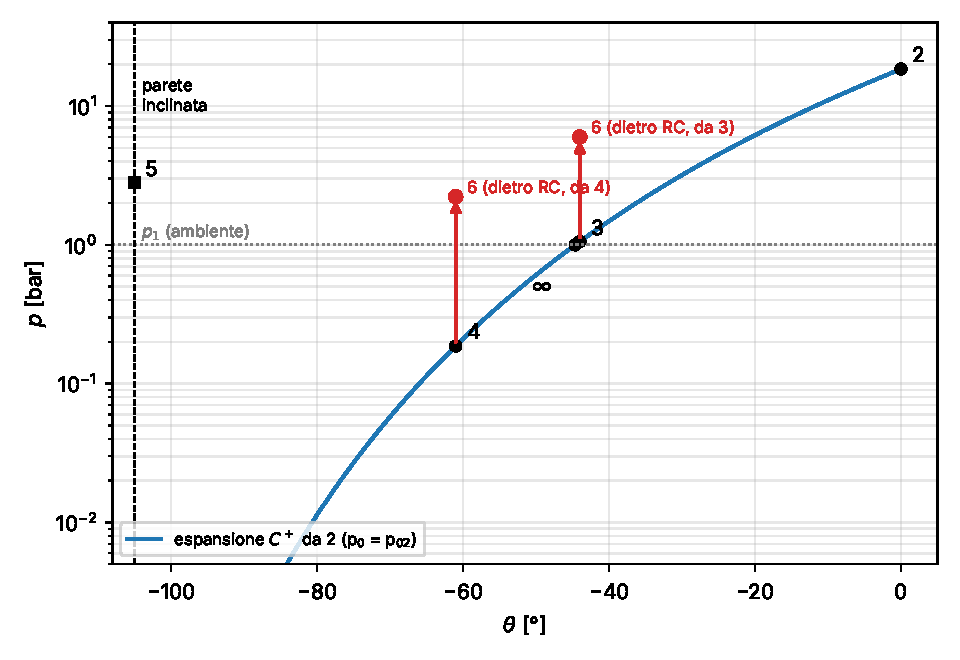
\includegraphics[width=0.7\textwidth]{p_theta_log.pdf}\\[4pt]
  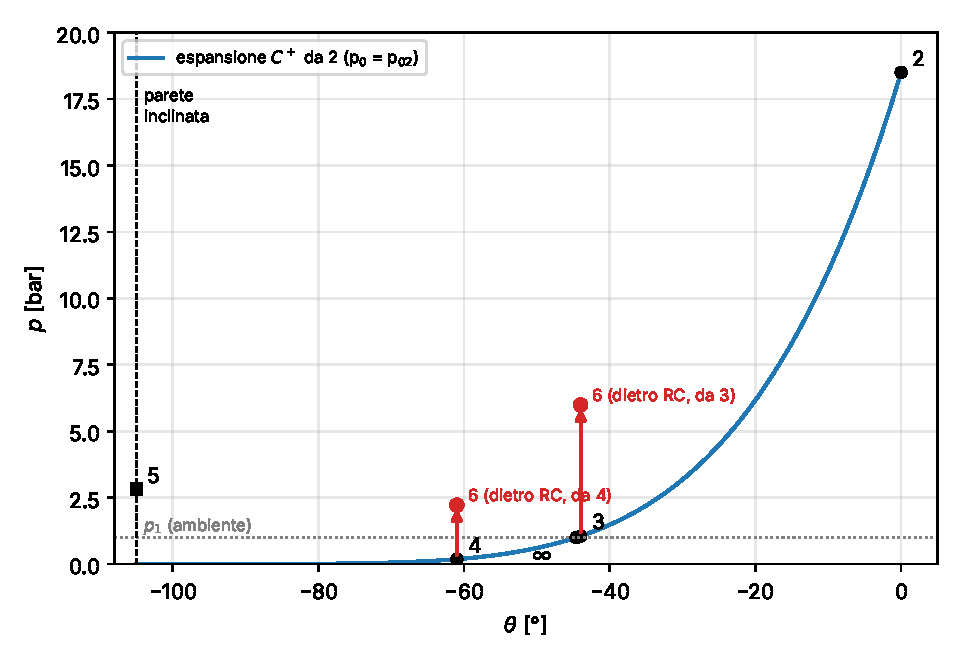
\includegraphics[width=0.7\textwidth]{p_theta_lin.pdf}
  \caption{Piano $p$--$\theta$ (sopra in scala logaritmica, sotto lineare): espansione $\Cp$ da 2, stati 3, 4,
  punto asintotico $\infty$, salti di RC (frecce rosse) e stato 5 alla direzione della parete inclinata.}
  \label{fig:pt}
\end{figure}

La figura annotata (fig.~\ref{fig:ann}) è la topologia del campo: stati, fronti dei ventagli, cerchio acustico dello
spigolo e punto D; la fig.~\ref{fig:lc} dà le linee di corrente.

%==============================================================================
\section{Coerenza con l'immagine e discussione}
\begin{itemize}
  \item \textbf{Calcolo e immagine concordano} sulla testa del ventaglio ($40^\circ$), sul punto E e sulla geometria
  di RC (arco quasi concentrico a C, alla distanza di B, che si indebolisce salendo). La zona scura della schlieren è il
  ventaglio di C: lì la densità cala fortemente (da $\rho_2$ a $\approx\rho_2/8$ nello stato 3).
  \item \textbf{Intensità di DS lungo il fronte.} Con la stessa regola $W_n=W\,h/x_A$ applicata alla tangente a DS
  ottengo il Mach locale dell'urto: $\approx4$ fino a D, $\approx3$ dove la normale è a $-40^\circ$, $\approx2{,}6$ a
  $-55^\circ$, $\approx2$ nel punto più basso e $1{,}6$ al piede ($p/p_1$ dietro l'urto da $18{,}5$ a $2{,}8$). DS è
  curvo e di intensità variabile, quindi lascia salti di entropia diversi su ogni linea di corrente e un campo
  rotazionale dietro di sé (Crocco); per questo le zone fra DS, CD e RC non sono uniformi.
  \item \textbf{Separazione.} Nel modello non viscoso la corrente 2 potrebbe in teoria girare di tutti i $105^\circ$
  ($\nu(M_2)+105^\circ<\nu_{max}$), ma arriverebbe a $M\approx24$ e $p\approx\SI{0.5}{Pa}$: la corrente reale si separa
  nello spigolo vivo e la deviazione è fissata dalla pressione della bolla. È l'unico punto in cui il campo non è
  determinato dalle sole equazioni di Eulero, e per questo $\theta_1$ e $\theta_2$ sono dati come misure.
  \item \textbf{Sovraespansione e ricompressione.} La seconda deviazione in F porta la corrente molto sotto
  l'ambiente ($p_4\approx0{,}19\,p_1$, $T_4\approx\SI{319}{K}$ contro $T_2=\SI{1186}{K}$): la ricompressione con RC
  è inevitabile e avviene con un urto intenso ($p_6/p_4\approx12$), con forte perdita di pressione totale.
  \item \textbf{Campo asintotico.} Il primo tratto di SL è già quello asintotico: è la regione ``più vecchia'' del
  campo autosimile. Il ventaglio in F, RC, CD e il vortice si allontanano dallo spigolo crescendo in proporzione al
  tempo; a lungo andare resta lo spigolo con l'espansione stazionaria fino a $p_1$ e la linea di separazione a
  $\approx44^\circ$.
  \item \textbf{Limiti.} Il vortice e lo strato di scorrimento sono viscosi e non si ricavano dal modello; le
  intensità di RC dipendono dalla velocità di RC, stimata con l'autosimilarità, e da quale stato lo attraversa, quindi
  sono stime. Gli stati 2, 3, 4, 5 e il campo asintotico sono invece esatti nel modello, a partire dai dati.
\end{itemize}

\end{document}
